% --------------------------------------------------------------- %
%             2. PASKIRSTYTŲ DIDŽIAKNYGIŲ TECHNOLOGIJOS
% --------------------------------------------------------------- %

\section {Paskirstytų didžiaknygių technologijos}

Kadangi problemos tiekimo grandinėse yra nepašalintos, reiškia, kad tradiciniai sprendimai ir technologijos, naudojamos jose vis dėlto neveikia taip gerai, kaip norėtųsi. Tačiau bet kuriuo atveju, norint vykdyti įmonės apskaitą ir talpinti įrašus ar transakcijas, teks naudotis didžiaknygės (angl. \textit{Ledger}) paslaugomis. O tas, kas teikia didžiaknygės paslaugas, turės įgyvendinti duomenų bazę, kad būtų galima valdyti duomenis.

Tačiau pagrindinė problema kyla dėl to, kad dalyvaujant pirkėjams ir pardavėjams, bei fiksuojant atliekamas transakcijas, yra reikalingas tarpininkas \cite{gao2018coc}, kuriuo pasitikėtų visos sistema besinaudojančos šalys. Didžiaknygės centralizuotas valdytojas savaime tampa vienvaldžiu tarpininku ir vieninteliu tiesos šaltiniu (angl. \textit{Single source of truth}), o tai suteikia perteklinę įtaką ir galią įrašų manipuliavimui bei kitas potencialias grėsmes \cite{jiang2017much} \cite{shyamasundar2018blockchain}. 

Vienas populiariausių didžiaknygės tarpininko pavyzdžių – bankas. Bankai yra tarpininkai tarp skirtingų šalių, kurios nori atlikti transakcijas tarpusavyje bei laikyti įrašus apie turimą turtą. Bankai sėkmingai gyvuoja dėl to, kad naudotojai, neturėdami kitos išeities ar alternatyvų, pasitiki jais. Tačiau šis pasitikėjimas turi ir savų rizikų. Bankinė institucija potencialiai gali susikompromituoti ir pradėti keisti, ištrinti įrašus savo naudai, taikyti mokesčius už tarpininkavimą ir pasisavinti turtą \cite{shyamasundar2018blockchain}. Tai yra priežastys, dėl kurių didžiaknygių naudotojai negali iki galo pasikliauti tokiais tarpininkais.

Neseniai vis daugiau susidomėjimo susilaukė paskirstytos didžiaknygės technologija (angl. \textit{Distributed Ledger Technology}), toliau – DLT. Pagrindinė priežastis, kodėl ji atkreipė rinkos, o ypač tiekimo grandinėse ir logistikoje esančių dalyvių dėmesį, yra jos technologinė prasmė. Vienai šaliai priklausanti centralizuota didžiaknygė pakeičiama į paskirstytą didžiaknygę, kuri nepriklauso jokiam savininkui, tačiau visi tinklo nariai turi jos kopijas, o tai reiškia pagrindinės problemos sprendimą – pašalintą trečiųjų šalių poreikį \cite{shyamasundar2018blockchain}. DLT naudojamai sistemai nebereikia administravimo, o tuo pačiu ir tarpininko mokesčio. Galiausiai užtikrinamas skaidrumas, pašalinant tikimybę, kad tarpininkas piktavališkai išnaudos turimą galią.



% --------------------------------------------------------------- %
%                          2.1. DLT SAVYBĖS
% --------------------------------------------------------------- %

\subsection{DLT savybės}

Nors pagrindinis DLT išskirtinumas yra tarpininko pašalinimas, jos unikalumas ir ypatybės tuo neapsiriboja. Šią technologiją būtų logiška tirti iš reikalavimų perspektyvos, kurie kyla iš tikimo grandinėse dalyvaujančių suinteresuotų šalių poreikių. Pagrindiniai poreikiai bus panagrinėti, bei įvertinta, kokią naudą tų poreikių išpildymui gali atnešti DLT savybės.



% --------------------------------------------------------------- %
%                           2.1.1. GREITIS
% --------------------------------------------------------------- %

\subsubsection{Greitis}

Šio darbo įžangoje jau buvo pabrėžta, kokio dydžio ir masto informacijos srautai bei transakcijų kiekiai vyrauja tiekimo grandinėse. Naudojama didžiaknygė turėtų būti labai greita, t.y. gebėti apdoroti šimtus tūkstančių įrašų per labai trumpą laiko tarpą, tiek juos rašant, tiek nuskaitant. Šis rodiklis gali būti matuojamas transakcijų kiekiu per sekundę (angl. \textit{Transactions per second}), toliau – TPS, arba kaip greitai įrašas atsiduria didžiaknygėje. Natūralu, kad kuo ilgesnis laukimo laikas, tuo daugiau nuostolių gali patirti tokios didžiaknygės naudotojai. Ateityje šie rodikliai turėtų nenumaldomai augti dėl vis labiau pradedamo taikyti daiktų interneto \cite{kaur2018edge}. 

Vienas iš įrašų kūrimo pavyzdžių – radijo dažnio identifikavimo (angl. \textit{Radio Frequency Identification}) technologijos, toliau – RFID. Jeigu kiekviename konteineryje, maisto plantacijose, fabrikuose ir t.t. būtų naudojamas vienas ar keli RFID davikliai, kurie paneštų savo būseną numatytu laiko periodu, tai reikštų milijardinius duomenų kiekius per parą pasauliniu mastu.

Be to, visi šie duomenys turėtų būti saugomi ilgą laiką. Įmonėms gali prireikti prieš kelis metus atliktų transakcijų, vykdytų operacijų ar RFID daviklių istorinių duomenų. Svarbus ir duomenų atsekamumas, kad būtų galima stebėti krovinių kelionę ir būseną, net jei šie duomenys buvo kaupiami tam tikrose vietose neturint interneto ryšio. Greitas ir stabilus visų šių duomenų valdymas tampa be galo sudėtingu IT infrastruktūriniu uždaviniu.

Nors duomenų apdorojimo greitis yra ko gero svarbiausias kriterijus, į kurį turi atsižvelgti technologijos, DLT iš savęs nepateikia sprendimo greičio klausimui spręsti. Tai – konkrečios DLT architektūros klausimas, nuo kurios ir priklauso, kokie sprendimai bus įgyvendinami, norint išpildyti greičio reikalavimus.

Tradicinės didžiaknygių sistemos iš esmės yra išsprendusios greičio klausimus ir gali apdoroti tūkstančius transakcijų per sekundę\footnote{Mokėjimų platformos, tokios kaip PayPal, vykdo apie 136 TPS, o Visa nuo 2 tūkst. TPS iki 56 tūkst. TPS \cite{herrera2016privacy}.} ar net milijonus transakcijų per sekundę \footnote{Šiuos rodiklius demonstruoja duomenų bazių valdymo sistemos, tokios kaip Oracle: https://blogs.oracle.com/timesten/scaling-sql-to-millions-of-transactions-per-second-with-a-single-database. Žiūrėta 2019-05-14.}. Tačiau naudojant DLT, dėl savo subtilybių ir specifikos, greičio problemos atsiranda kitu pavidalu. Kiekvieno įrašo padarymas yra konsensuso algoritmo (angl. \textit{Consensus Algorithm}) dalis. Konsensuso algoritmas – tai protokolas, kuris pasirūpina, kad visi tinklo nariai sinchronizuotųsi tarpusavyje ir prieitų bendrą sutarimą įvertinant, kurios transakcijos yra tinkamos, kad jas būtų galima pridėti į didžiaknygę \cite{cachin2017blockchain}. 



% --------------------------------------------------------------- %
%                     2.1.2. DUOMENŲ NEKINTAMUMAS
% --------------------------------------------------------------- %

\subsubsection{Duomenų nekintamumas}

Tiekimo grandinėse ypatingai svarbu, kad įrašai nebūtų padirbinėjami arba sunaikinami be žinios. Šiuo metu vyraujant centralizuotoms duomenų bazėms, administratoriai gali manipuliuoti duomenimis, o fizinės duomenų saugyklos įvykus nenumatytiems incidentams gali būti pažeistos nepataisomai.

DLT siūlo decentralizuotos didžiaknygės architektūrą (žr. 5 pav.), kurios veikimui nereikia jokios centralizuotos duomenų saugyklos ar administravimo \cite{yu2018virtualization}. Didžiaknygė tampa paskirstyta visame tinkle ir, naudojant konsensuso algoritmą, visi autorizuoti pakeitimai bet kurio vartotojo didžiaknygės kopijoje atsispindi visų tinkle esančių vartotojų kopijose \cite{puthal2018blockchain}. 

\begin{figure}[H]
    \centering
    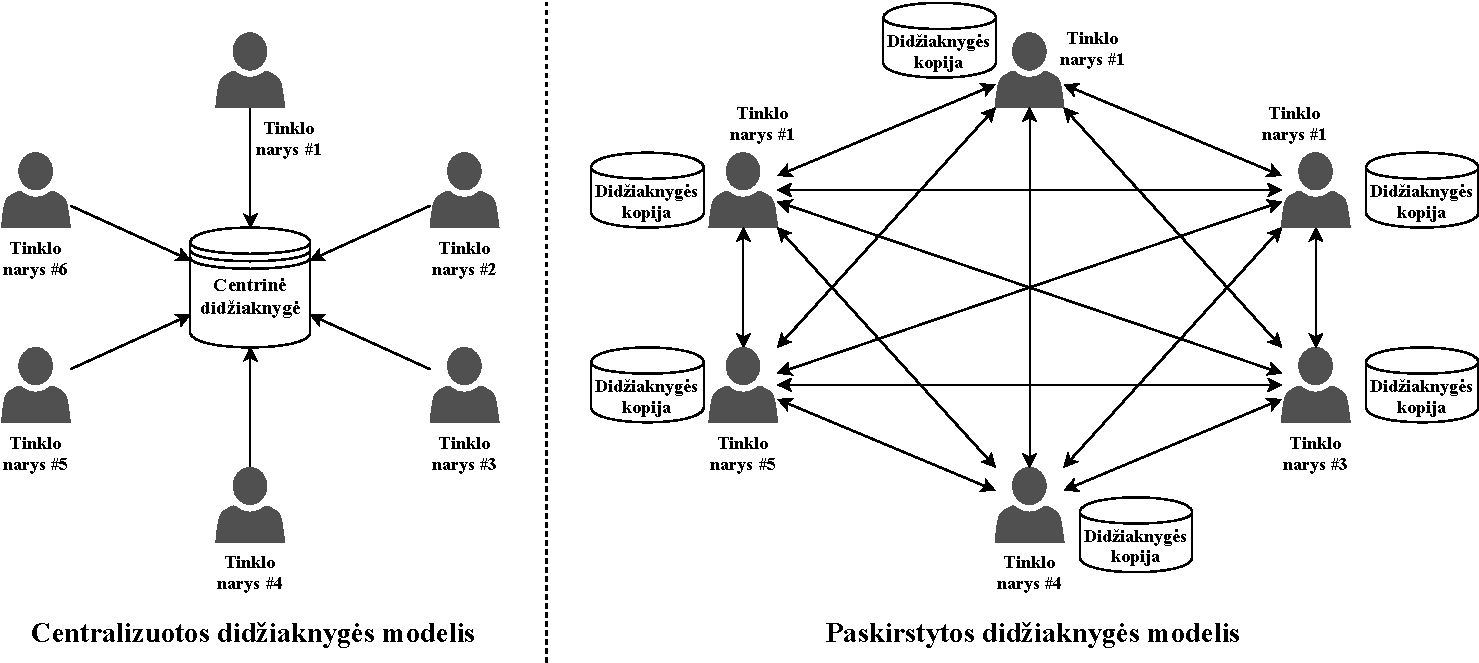
\includegraphics[scale=0.65]{images/ledger-model-types}
    \caption{Didžiaknygių tipų modeliai}
\end{figure}

Iš to kyla viena svarbiausių DLT savybių: tai, kas įrašyta į paskirstytą didžiaknygę, negali būti pakeista arba ištrinta – šitaip yra pasiekiamas duomenų nekintamumas (angl. \textit{Data Immutability}) \cite{xu2017dl}. Tokiu atveju visi duomenys tampa apsaugoti nuo potencialaus duomenų padirbinėjimo. O tai leidžia matyti visą unikalią istorinę informaciją. Pavyzdžiui, transportuojant prekes iš taško A į tašką B ir fiksuojant krovinio vietą laike, galime matyti visą jo kelionės istorinę informaciją ir pasitikėti paskirstyta didžiaknyge, jog tie duomenys yra autentiški. 

Tą užtikrina jau minėtas konsensuso algoritmas, apsaugantis duomenis nuo piktavalių naudotojų. Tačiau ši savybė tam tikrais atvejais gali būti tuo pačiu ir trūkumas. Pavyzdžiui, kai naudojame dinamiškai besikeičiančią informaciją, galinčią dažnai kisti. Pasikeitus kliento mobilaus telefono numeriui, atnaujinti esamo duomenų įrašo negalėtume ir tektų kurti naują įrašą apie atsinaujinusius kliento duomenis.



% --------------------------------------------------------------- %
%                       2.1.3. DUOMENŲ SAUGUMAS
% --------------------------------------------------------------- %

\subsubsection{Duomenų saugumas}

Svarbu, kad privatūs ir jautrūs duomenys, kuriais disponuoja įmonės, būtų apsaugoti, o prieigą prie jų turėtų tik tie, kam duomenys priklauso arba turi leidimą juos valdyti. Tai tapo dar svarbesniu veiksniu 2018 metais įsigaliojus GDPR reglamentui \cite{ferrari2018eu}. Jeigu įmonės paviešintų tokią informaciją, ji patirtų milžiniškus piniginius nuostolius dėl baudų, o nutekinta įmonei svarbia informacija pasinaudotų jos konkurentai.

Didelė dalis populiariausių DLT yra viešos, nereikalaujančios prieigos teisių (angl. \textit{Permissionless Ledger}), t.y. visi vartotojai turi prieigą prie didžiaknygės \cite{olnes2017blockchain}. Šitaip viešai matoma kas ir kokią informaciją įrašo į paskirstytą žurnalą, o tuo pačiu bet kas gali kurti naujus įrašus. Tačiau galimos ir papildomos DLT konfigūracijos. Pavyzdžiui, galima sukurti tokią privačią paskirstytą didžiaknygę (angl. \textit{Permissioned Ledger}), kad duomenis skaityti bei rašyti galėtų tik prieigos teisę turinčios šalys \cite{backlund2016technical}. Tai yra naudinga, jeigu dvi ar daugiau įmonių yra verslo partneriai ir nori dalintis bendra informacija ar atlikti transakcijas tarpusavyje, tačiau jie nenorėtų, kad bet kas kitas už šio rato ribų apie tai žinotų. 

Tačiau duomenis apsaugoti galima ir kitais būdais. Pavyzdžiui, naudojant kriptografijos metodus, tokius kaip privatų ir viešą raktą \cite{zyskind2015decentralizing}, galime užšifruoti duomenis ir į paskirstytą didžiaknygę įrašyti tik tam tikrą maišos reikšmę. Tiesa, visi tinklo nariai matys kas šiuos duomenis patalpino, tačiau niekas nežinos kokie tai duomenys, išskyrus šalis, turinčias privatų raktą. Tai leidžia talpinti jautrią informaciją į viešą DLT ir jaustis saugiai, nes peržiūrėti jos originalų formatą be leidimo, t.y. privataus rakto, negali niekas.



% --------------------------------------------------------------- %
%                         2.2. DLT ATMAINOS
% --------------------------------------------------------------- %

\subsection{DLT atmainos}

Yra du pagrindiniai DLT tipai. Tai blokų grandinės (angl. \textit{Blockchain}) ir orientuoto grafo be ciklų (angl. \textit{Directed Acyclic Graph}), toliau – DAG struktūrą turintys DLT, kurie bus analizuojami tolimesniuose poskyriuose.



% --------------------------------------------------------------- %
%               2.2.1. BLOKŲ GRANDINĖS TECHNOLOGIJA
% --------------------------------------------------------------- %

\subsubsection{Blokų grandinės technologija}

Šiuo metu yra daug blokų grandinių projektų, tačiau populiariausiomis ir stabiliausiomis išlieka dvi – Bitcoin ir Ethereum\footnote{Duomenys paimti iš: https://coinmarketcap.com. Žiūrėta 2019-05-14.}. Šios blokų grandinės veikia tokiu principu: blokai, kuriuose saugoma informacija, t.y. transakcijos bei kitos blokų grandinei reikalingos reikšmės, yra sujungiami tarpusavyje į vieną ilgą ir nenutrūkstamą seką (žr. 6 pav.)\footnote{Paveikslėlyje pavaizduota architektūra yra prototipinė autoriaus sukurta blokų grandinė. Realybėje egzistuojančių blokų grandinių architektūros yra kur kas sudėtingesnės.}. Vienintelis būdas sukurti naujus įrašus – surinkti juos į naują bloką ir prijungti jį prie paskutinio grandinėje esančio bloko.

\begin{figure}[H]
    \centering
    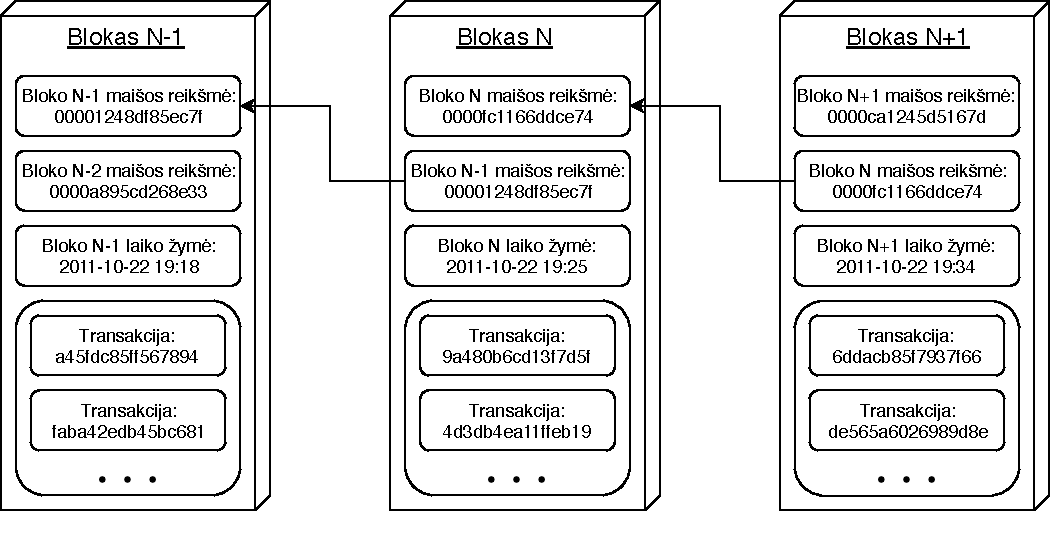
\includegraphics[scale=0.85]{images/block-chain-architecture}
    \caption{Blokų grandinės architektūrinis modelis}
\end{figure}



% --------------------------------------------------------------- %
%          2.2.1.1. BLOKŲ GRANDINĖS DUOMENŲ NEKINTAMUMAS
% --------------------------------------------------------------- %

\subsubsubsection{Blokų grandinės duomenų nekintamumas}

Jeigu bandytume pridėti bloką grandinės viduryje, ši išsišakotų į 2 atskiras šakas. Čia svarbią reikšmę turi konsensuso algoritmas. Konsensuso algoritmas turi apsaugoti blokų grandinę nuo grandinės išsišakojimų, blokų ištrynimo, keitimo, dvigubo išleidimo problemos (angl. \textit{Double-spending problem}) bei kitokių taisyklių pažeidimų ar spragų, kuriomis norėtų pasinaudoti kenkėjai tinkle \cite{baliga2017understanding}. Kitaip – garantuoti duomenų nekintamumą.

Vienas iš tokių konsensuso algoritmo atmainų, kurį naudoja Bitcoin ir Ethereum, yra įdėto darbo įrodymo (angl. \textit{Proof of Work}) konsensuso algoritmas, toliau – PoW \cite{gervais2016security}. Kaskart norint pridėti bloką, reikia atlikti darbą, kuris reikalauja kompiuterinių skaičiavimų galios, laiko ir energijos išteklių. Blokų grandinėje kuriant naujus blokus kartais atsiranda išsišakojimai. Tai įvyksta tada, jeigu du ar daugiau blokų iškasami beveik tuo pačiu metu \cite{zheng2017overview}. Atsiradus tokiems išsišakojimams, yra pasirenkama ilgiausia atšaka, t.y. tokia, kuri turi daugiausiai blokų \cite{zheng2017overview}. 

Tačiau išsišakojimus galima kurti ir savanaudiškais tikslais. Tinklo kenkėjas, norintis pakeisti transakciją viename iš blokų, sukurs grandinės išsišakojimą. Tačiau tam, kad tinklas pripažintų pakeistą transakciją grandinėje, kenkėjas turės atlikti darbą, kurį padarė visas tinklas nuo išsišakojimo pradžios iki einamojo momento \cite{nakamoto2008bitcoin}. Be to, atlikti PoW darbą reikės gerokai sparčiau nei visi kiti tinklo nariai kartu sudėjus, kad kenkėjas ne tik pasivytų visą tinklą grandinės ilgiu, bet ir jį aplenktų, kad jo grandinės išsišakojimas taptų ilgesnis už pagrindinę grandį \cite{nakamoto2008bitcoin}\footnote{Šis scenarijus dar yra vadinamas 51 procento ataka (angl. \textit{51\% Attack)} \cite{baliga2017understanding}.}. Tik tokiu atveju piktybinę grandį tinklas priimtų kaip teisingą (žr. 7 pav.).

Šiuo metu tiek Bitcoin, tiek Ethereum toks scenarijus yra labai mažai tikėtinas, nes naujus blokus sukuria didelis kiekis kasėjų (angl. \textit{Miners}), kuriems PoW suteikia stimulą (angl. \textit{Incentive}) kasti, t.y. kurti naujus blokus. Tą lemia PoW skatinimo sistema: už kiekvieną iškastą bloką yra skiriamas apdovanojimas – kripto valiuta (angl. \textit{Cryptocurrency}) \cite{nakamoto2008bitcoin}. Taigi, tinklo kenkėjui beveik nėra šansų pakreipti konsensuso algoritmo savo naudai – tai tiesiog neapsimoka ir beveik neįmanoma techniškai. Šitaip užtikrinamas vienas iš reikalavimų – duomenų patvarumas ir nesuklastojamumas.

\begin{figure}[H]
    \centering
    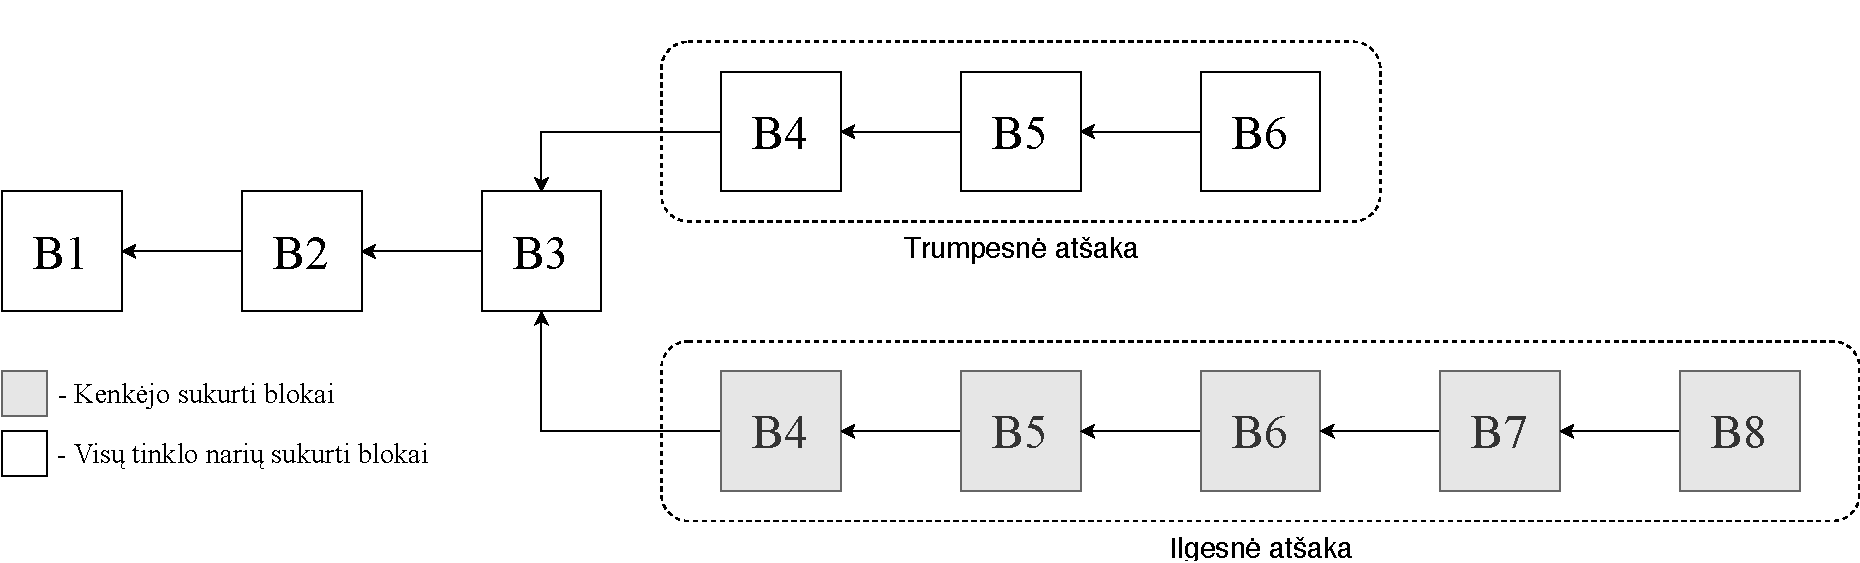
\includegraphics[scale=0.5]{images/blockchain-branches}
    \caption{Blokų grandinės šakos}
\end{figure}



% --------------------------------------------------------------- %
%               2.2.1.2. BLOKŲ GRANDINĖS PRALAIDUMAS
% --------------------------------------------------------------- %

\subsubsubsection{Blokų grandinės pralaidumas}

Blokų grandinės pralaidumas (angl. \textit{Throughput}) priklauso nuo daugelio faktorių. Visi šie faktoriai yra susiję su transakcijų gyvavimo ciklu. Bitcoin atveju transakcijų gyvavimo ciklas veikia tokiu principu \cite{nakamoto2008bitcoin}:
\begin{enumerate}
    \item Visų pirma, kiekvienas narys, sukurdamas transakciją, ją viešai paskelbia kitiems tinklo nariams. 
    \item Bloko kasėjas surenka dalį arba visas viešai paskelbtas transakcijas į bloką ir atlieka darbą pagal PoW konsensuso algoritmą.
    \item Apskaičiavęs darbo rezultatą kasėjas paskelbia naujai sukurtą bloką visiems tinklo nariams viešai. 
    \item Jeigu kiti tinklo nariai pasitiki bloke esančių transakcijų tinkamumu, blokas galiausiai prijungiamas prie visos grandinės pabaigos ir tinklas nuosekliai jungia naujus blokus prie šio bloko. 
\end{enumerate}

Tačiau tuo bloko gyvavimo ciklas nesibaigia. Jeigu blokas prijungiamas prie grandinės, dar nereiškia, kad jis laikomas patvirtintu. Tam, kad blokas būtų laikomas saugiai patvirtintu, o kartu su juo ir transakcijos jame, prie šio bloko nuosekliai dar turi būti prijungtas tam tikras kiekis blokų. 

Taip pat yra tikimybė, kad transakcija nebus patvirtinta, jeigu blokų kasėjai jos neįtrauks į blokus. Blokų kasėjai renkasi transakcijas pagal tai, kokią jie naudą gaus pridėdami jas į bloką. Ši nauda matuojama transakcijos mokesčiu (angl. \textit{Transaction fee}), kurį nurodo transakcijos kūrėjas. Taigi, gali atsitikti taip, kad, transakcijos kūrėjas pasiūlys per mažą kainą už savo transakcijos įtraukimą į bloką ir ji niekada nebus patvirtinta.

Taigi matome, kad transakcijų greitis priklauso nuo šių pagrindinių priežasčių: 
\begin{itemize}
    \item Kiek laiko trunka bloko sukūrimas, kitaip – per kiek laiko atliekamas PoW skaičiavimas.
    \item Kiek blokas gali talpinti savyje transakcijų, arba kitaip bloko dydis baitais.
    \item Kiek reikalinga tolimesnių blokų, kad blokas būtų laikomas saugiai patvirtintu.
    \item Mokesčio dydžio, kuris lemia, kad kasėjai įtrauks transakciją į bloką su beveik 100\% tikimybe.
\end{itemize} 

Žemiau pateikiama lentelė (žr. 1 lentelė) su Bitcoin ir Ethereum platformų rodiklių palyginimais. Iš joje esančių duomenų seka maksimalus TPS greitis.

\begin{longtable}{|L{3,8cm}|L{5,3cm}|L{6cm}|}
\caption{Bitcoin ir Ethereum rodiklių palyginimas}
\label{variability_impl_mech}
\endfirsthead
\endhead
\hline
\textbf{Palyginimo kriterijus} & \multicolumn{1}{c|}{\textbf{Bitcoin}} & \multicolumn{1}{c|}{\textbf{Ethereum}} \\ \hline
\textbf{Transakcijų kiekio bloke limitas} & Apie 4000 transakcijų \cite{zhu2016interactive} & 380 unikalių transakcijų limitas\footnote{Bloko GAS limitas – 8 mln. \cite{hu2018hierarchical}, o vienos transakcijos minimalus GAS limitas – 21 tūkst. \cite{xu2017taxonomy}. Todėl 8000000 / 21000 = 380.} \\ \hline
\textbf{Bloko iškasimo laikas} & 10 min. \cite{macdonald2017blockchain} & 10-20 sekundžių \cite{gervais2016security} \\ \hline
\textbf{Patvirtinimo blokų kiekis} & 6 \cite{xu2017taxonomy} & 12 \cite{xu2017taxonomy} \\ \hline
\textbf{Saugaus patvirtinimo laikas} & 1 valanda \cite{xu2017taxonomy} & 3 minutės \cite{xu2017taxonomy}  \\ \hline
\textbf{Vidutinė transakcijos mokesčio kaina} & ?\footnote{TODO} & ?\footnote{TODO} \\ \hline
\textbf{TPS limitas} & 7 TPS \cite{macdonald2017blockchain} & 25 TPS \cite{bocek2018smart} \\ \hline
\end{longtable}



% --------------------------------------------------------------- %
%                 2.2.1.3. BLOKŲ GRANDINIŲ TRŪKUMAI
% --------------------------------------------------------------- %

\subsubsubsection{Blokų grandinių trūkumai}

1 lentelėje pateikti duomenys akivaizdžiai parodo blokų grandinių trūkumus. Žinant tiekimo grandinių ir logistikos mastus, šiuo metu šios platformos neturėtų šansų patenkinti rinkos poreikių dėl esamų suvaržymų: 
\begin{itemize}
    \item TPS limitai. Būtų sunku įsivaizduoti didelių sistemų funkcionavimą bent vienoje iš šių platformų, nes jos paprasčiausiai nesusitvarkytų su milijoniniais atliekamų transakcijų kiekiais. Logistikoje yra įprasta, kad vien individualios siuntos kelionės gyvavimo cikle dažnai pasikeičiant savininkams, yra atliekama keletas ar net dešimtys transakcijų.
    \item Patvirtinimo laukimo laikas. Tiekimo grandinėse kiekviena minutė yra svarbi ir kainuoja. Laukti kelioliką minučių ar net valandą, kol transakcija bus patvirtinta, stabdytų įprastą tiekimo grandinės tėkmę ir atneštų didelių nuostolių. Be to, naudojant blokų grandines egzistuoja tikimybė, kad transakcija taip ir nebus įtraukta į blokų grandinę.
    \item Mokesčiai už atliekamas transakcijas tikriausiai yra vienas iš labiausiai atbaidančių suvaržymų. Tikėtina, kad tam tikrais atvejais mokesčiai už transakcijas gali būti aukštesni už transportuojamų prekių kainą.
\end{itemize} 

Tam tikros blokų grandinės yra įgyvendinusios išmaniųjų kontraktų (angl. \textit{Smart contracts}) funkcionalumą, kuris praturtina technologijos potencialą ir savaime yra privalumas. Išmanieji kontraktai – sistemos, kurios automatiškai įvykdo veiksmus pagal prieš tai aprašytas taisykles \cite{buterin2013ethereum}.

Ethereum išmanieji kontraktai įgalina automatizuotus kriptovaliutų pervedimus pagal programinį kodą, remiantis sugalvotais scenarijais. Tačiau jų realizavimas praktikoje kol kas atrodo neefektyvus. Visi tinklo nariai, norintys patikrinti bloko validumą, turintį savyje transakciją, kuri inicijuoja išmaniojo kontrakto vykdymą, turi vykdyti tą patį išmaniojo kontrakto kodą \cite{buterin2013ethereum}. Dėl šios priežasties vienos programos, paremtos išmaniuoju kontraktu išpopuliarėjimas apkrovė ir smarkiai sulėtino Ethereum tinklą\footnote{https://cryptovest.com/news/ethereum-loses-to-cryptokitties-network-remains-slow. Tikrinta 2019-05-14.}.



% --------------------------------------------------------------- %
%                      2.2.2. DAG TECHNOLOGIJA
% --------------------------------------------------------------- %

\subsubsection{DAG technologija}

Šiuo metu egzistuoja gerokai mažiau DAG principu paremtų projektų, palyginus su blokų grandinės projektais. Tačiau vienas iš įdomiausių ir daugiausiai žadančių – IOTA platforma. 



% --------------------------------------------------------------- %
%                   2.2.2.1. IOTA VEIKIMO POBŪDIS
% --------------------------------------------------------------- %

\subsubsubsection{IOTA veikimo pobūdis}

Vietoje blokų grandinės ir joje kasamų blokų su transakcijomis, IOTA įgyvendino DAG struktūrą turinčią paskirstytą didžiaknygę, vadinamą raizginiu (angl. \textit{Tangle}) (žr. 8 pav.). Modelyje vaidmenį atlieka 3 elementai:
\begin{itemize}
    \item Patvirtinta transakcija. Tai tokia transakcija, kurią patvirtina bent 1 kita transakcija.
    \item Nepatvirtinta transakcija. Jos dar vadinamos raizginio viršūnėmis (angl. \textit{Tips}). Šios transakcijos jokia kita transakcija dar nepatvirtino.
    \item Transakcijos patvirtinimas. Kiekvienas IOTA tinklo narys, norėdamas atlikti transakciją, privalo patvirtinti kitas 2 transakcijas \cite{popov2016tangle}.
\end{itemize} 

\begin{figure}[H]
    \centering
    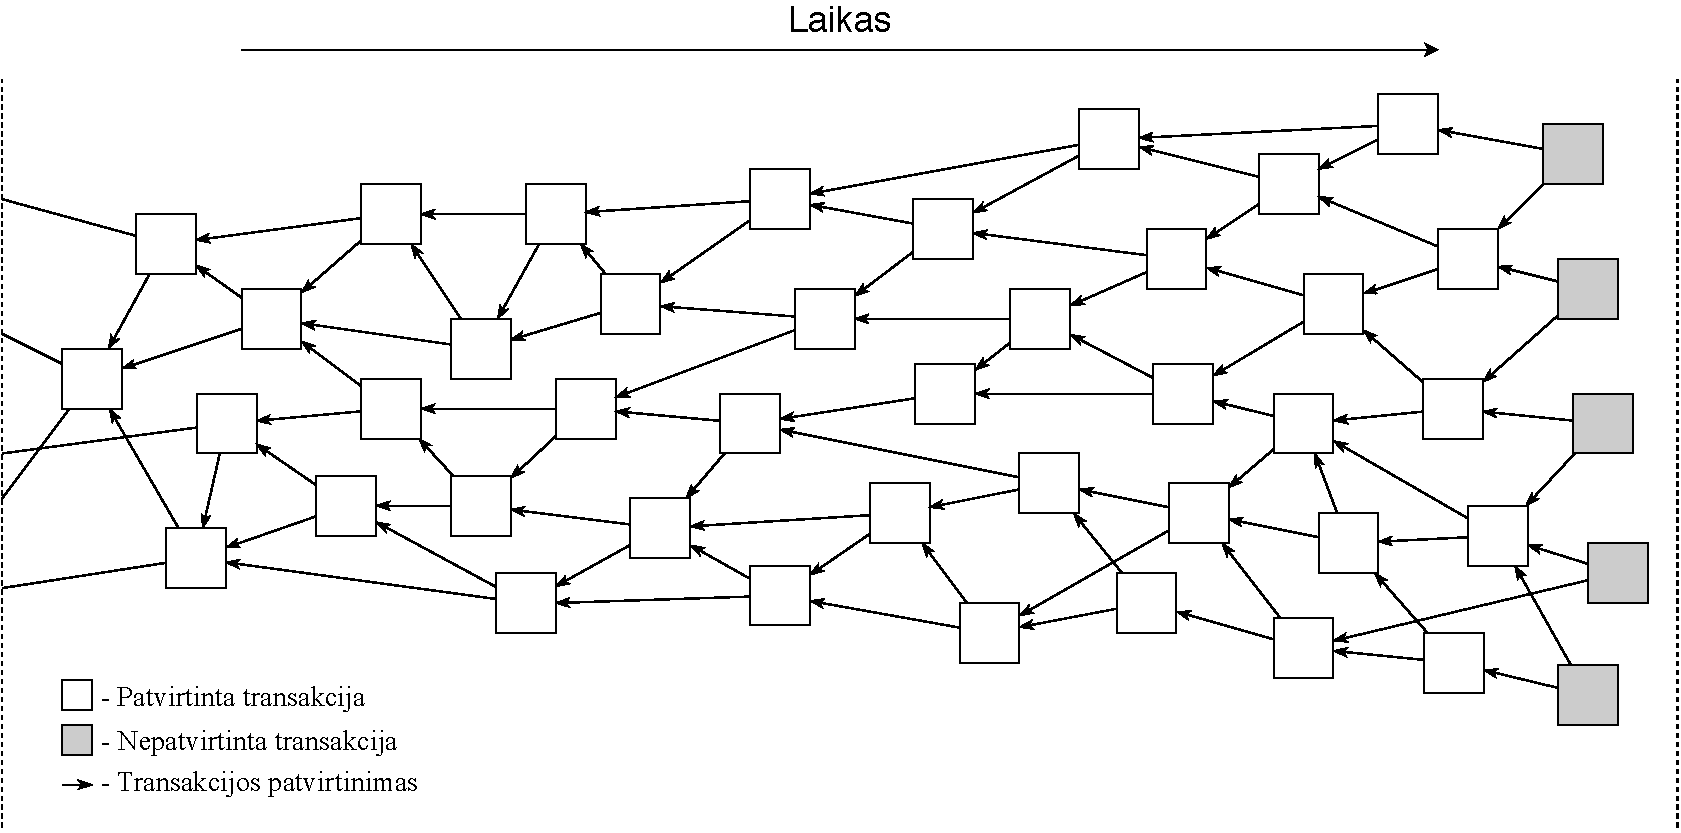
\includegraphics[scale=0.56]{images/iota-tangle}
    \caption{IOTA raizginio modelis}
\end{figure}

Transakcijų patvirtinimo įgyvendinimas yra unikalus ir specifinis procesas, kuriame didelę reikšmę turi matematiniai skaičiavimai. Visų pirma, norint atlikti transakciją IOTA tinkle, yra privaloma atlikti nuoseklius žingsnius: pasirinkti 2 transakcijas, patikrinti jų validumą (dvigubo išleidimo problema) ir atlikti darbą PoW principu \cite{popov2016tangle}. 

Unikalu yra tai, kad kiekvienas narys, norintis atlikti transakciją, PoW atlieka pats \cite{bramas2018stability}. Priešingai negu Bitcoin ar Ethereum, kur PoW galima deleguoti kitiems tinklo nariams, už tai sumokant transakcijos mokestį. Tačiau IOTA naudojamas PoW yra gerokai paprastesnis ir nereikalaujantis daug skaičiavimo galios \cite{popov2016tangle}. Visų pirma, PoW reikalingas tam, kad būtų apsisaugoma nuo fiktyvių transakcijų (angl. \textit{Spam}) \cite{popov2016tangle}. Skaičiavimų sudėtingumas žemas dėl to, kad IOTA pritaikyta daiktų internetui, kuriame dalyvauja labai smulkūs prietaisai, neturintys pajėgumų sudėtingiems skaičiavimams atlikti.

Tuo tarpu transakcijų parinkimo klausimas nėra toks trivialus ir nuo to priklauso visos ekosistemos stabilumas. IOTA ir neturi jokių formalių taisyklių transakcijų parinkimo patvirtinimui, t.y. galima laisva nuožiūra pasirinkti pačiam, kokias transakcijas patvirtinti \cite{popov2016tangle}. Tačiau egzistuoja rekomendacinis algoritmas \cite{popov2016tangle}. Šį algoritmą renkasi dauguma tinklo narių, nes daugumai sąžiningai jo laikantis padidėja tikimybė, kad likę nariai taip pat laikysis šio algoritmo. Iš to seka, kad algoritmo besilaikančių narių transakcijos bus patvirtintos kitų narių su aukštesne tikimybe.

2 transakcijos parenkamos pagal galūnių parinkimo algoritmą (angl. \textit{Tip Selection Algorithm}), toliau – TSA, o IOTA atveju konkrečiai – Markov Chain Monte Carlo (MCMC) algoritmu, kurio veikimui įtaką daro su kiekviena transakcija susieta informacija ir atributai \cite{bramas2018stability}. Tai transakcijos svoris (angl. \textit{Weight}), transakcijos taškai (angl. \textit{Score}) ir transakcijos kaupiamasis svoris (angl. \textit{Cumulative Weight}) \cite{popov2016tangle}. 



% --------------------------------------------------------------- %
%                       2.2.2.2. IOTA SAUGUMAS
% --------------------------------------------------------------- %

\subsubsubsection{IOTA saugumas}

IOTA technologija buvo pradėta kurti atsižvelgus į ateities perspektyvas ir kuriamas naujas technologijas. Viena iš tokių ateities perspektyvų – kvantiniai kompiuteriai (angl. \textit{Quantum Computers}), kurie gali padaryti daugumą blokų grandinių pažeidžiamomis. Šis pažeidžiamumas kyla iš to, kaip yra atliekami PoW skaičiavimai ir pasirašomos transakcijos \cite{kiktenko2018quantum}. Pakankamai galingas kvantinis kompiuteris galėtų įvykdyti 51 procento ataką ir pakreipti visą tinklą savo naudai \cite{kiktenko2018quantum}. 

Tai reiškia, kad Bitcoin, o kartu ir visos PoW konsensuso algoritmu paremtos blokų grandinės taptų nesaugios. Tačiau net jeigu blokų grandinė ir nėra paremta PoW konsensuso algoritmu, ji gali tapti nesaugi ir kitomis prasmėmis. Tam tikrais atvejais yra būtina paviešinti viešą raktą ir kvantinis kompiuteris, pasinaudojęs šiuo raktu, galėtų nustatyti privataus rakto reikšmę \cite{aggarwal2017quantum}. Privatus raktas yra naudojamas pasirašant transakcijas, patvirtinant savo tapatybę bei laikant kriptovaliutas (angl. \textit{Cryptocurency}) kripto piniginėse (angl. \textit{Crypto Wallets}). Tokia spraga reikštų, kad asmenys, disponuojantys kvantiniu kompiuteriu, galėtų perskaityti privačiu raktu užšifruotas žinutes, pasisavinti sąskaitoje laikomą turtą ar apsimesti kitu asmeniu.

IOTA savo ruožtu nepateikia visiško atsparumo kvantinių kompiuterių atakoms, tačiau teigia, kad jų sprendimas yra žymiai saugesnis, negu Bitcoin ar kitų panašių platformų. IOTA naudoja Winternitz vienkartinę parašo panaudojimo schemą, kuri, kaip manoma, yra atspari kvantiniams kompiuteriams \cite{el2018review}.



% --------------------------------------------------------------- %
%                     2.2.2.3. IOTA PRALAIDUMAS
% --------------------------------------------------------------- %

\subsubsubsection{IOTA pralaidumas}

IOTA, priešingai negu blokų grandinės, neturi tokio architektūrinio vieneto kaip blokas, todėl pralaidumas ir greitis priklauso tik nuo individualių transakcijų patekimo į raizginį greičio. Žinant IOTA veikimo principą, galima išskirti rodiklius, darančius įtaką tinklo pralaidumui:
\begin{itemize}
    \item PoW skaičiavimo atlikimo laikas;
    \item Kokia tikimybė, kad transakciją patvirtins kiti nariai;
    \item Kiek ilgai kitiems tinklo nariams užtrunka patikrinti transakcijos validumą ir ją patvirtinti;
    \item Kiek tinkle yra aktyvių narių, kuriančių transakcijas.
\end{itemize}

IOTA neturi konkrečių teorinių TPS limitų. Visi apribojimai kyla iš to, kaip greitai individualių transakcijų kūrėjai apskaičiuos kiekvienai transakcijai reikalingą atlikti PoW. Taip pat, kuo daugiau aktyvių narių tinkle, tuo aukštesnis bendras TPS dydis, nes daugiau narių kuria naujas transakcijas ir daugiau narių jas tvirtina. Taigi vieninteliai technologijos limitai – tai individualių mašinų tinkle kiekis bei jų skaičiavimo ir validavimo sparta.

Kitas svarbus aspektas – transakcijų mokestis. IOTA netaiko jokio transakcijų mokesčio \cite{zivic2019distributed}. O tai tampa pranašumu tinklo naudotojams, kurio neturi dauguma blokų grandinių ir net VISA naudotojų. Be to, transakcijos neprivalo perduoti kriptovaliutų. Tai reiškia, kad galima atlikti tuščias transakcijas arba tiesiog dalintis informacija su kitais tinklo nariais. Ši savybė tampa naudinga daiktų internetui atliekant mikrotransakcijas.



% --------------------------------------------------------------- %
%        2.2.2.4. PASLĖPTI NUSTATYTOS TAPATYBĖS PRANEŠIMAI
% --------------------------------------------------------------- %

\subsubsubsection{Maskuotieji nustatytos tapatybės pranešimai}

Tiekimo grandinėse nepaprastai svarbu duomenų atsekamumas. Daugumai grandinės narių svarbu matyti prekės judėjimą, t.y. kur ir kada prekė keliavo, kaip pasikeitė prekės laikinieji savininkai, kokia buvo prekės būsena skirtingais laiko momentais ir t.t. Be to, kai kurie duomenys yra jautrūs ir reikia suvaldyti kuri informacija kurioms šalims turi būti prieinama, o kuri – ne. Šį darbą dažnai tenka atlikti ranka, patikrinant skirtingus informacijos šaltinius.

IOTA šiai problemai spręsti yra sukūrusi paslėptus nustatytos tapatybės pranešimus (angl. \textit{Masked Authenticated Message}), toliau – MAM. Tai yra biblioteka, užšifruojanti, iššifruojanti ir nustatanti tapatybę duomenų, kuriuos yra norima publikuoti į IOTA raizginį \cite{andreas2017masked}. Publikuojant tokius užšifruotus duomenis, galima atskleisti specialų raktą prenumeratoriams (angl. \textit{Subscribers}), kurie turėtų teisę stebėti duomenis. Duomenų pranešėjas (angl. \textit{Publisher}) tam sukuria kanalą (angl. \textit{Channel}) \cite{ab2018iota}.

Atidarius kanalą atsiranda nemažai konfigūracijos pasirinkimų. Kanalą galima padaryti išsišakojusį, kiekvieną šaką padaryti prieinamą skirtingoms šalims ir kiekvienoje jų publikuoti skirtingą informaciją \cite{ab2018iota}. Taip pat galima nustatyti norimą kanalo privatumo režimą iš 3 galimų rūšių \cite{paul2017introducing}:
\begin{itemize}
    \item Viešas (angl. \textit{Public}), kuriame skelbiama informacija yra prieinama absoliučiai kiekvienam IOTA tinklo nariui.
    \item Privatus (angl. \textit{Private}), kurį gali iššifruoti šalis, turinti specialų raktą. Naudinga įrenginių tarpusavio komunikacijai.
    \item Suvaržytas (angl. \textit{Restricted}), kurį gali iššifruoti šalis, turinti specialų raktą, bei turinti autorizacijos raktą. Šis režimas leidžia kanalo iniciatoriui nutraukti transliavimą šalims, turinčioms tam tikrą autorizacijos raktą nepakeičiant specialaus rakto reikšmės. Nustačius naują autorizacijos raktą galima nustatyti, kam bus suteiktos naujos prenumeratorių teisės.
\end{itemize}

Supaprastintas MAM veikimo modelis pavaizduotas 9 pav. Duomenų pranešėjas siunčia žinutes, kurias yra užsiprenumeravę 3 prenumeratoriai. Pirmajam pranešėjas atskleidė specialų ir autorizacijos raktą, todėl jis gali iššifruoti ir perskaityti visų kanalų žinutes. Antrasis prenumeratorius turi specialų raktą, todėl gali skaityti privataus ir viešo kanalo žinutes, tačiau negali iššifruoti suvaržyto kanalo žinutės. Trečiasis prenumeratorius gali skaityti tik viešojo kanalo žinutes, t.y. trečią ir šeštą žinutes.

\begin{figure}[H]
    \centering
    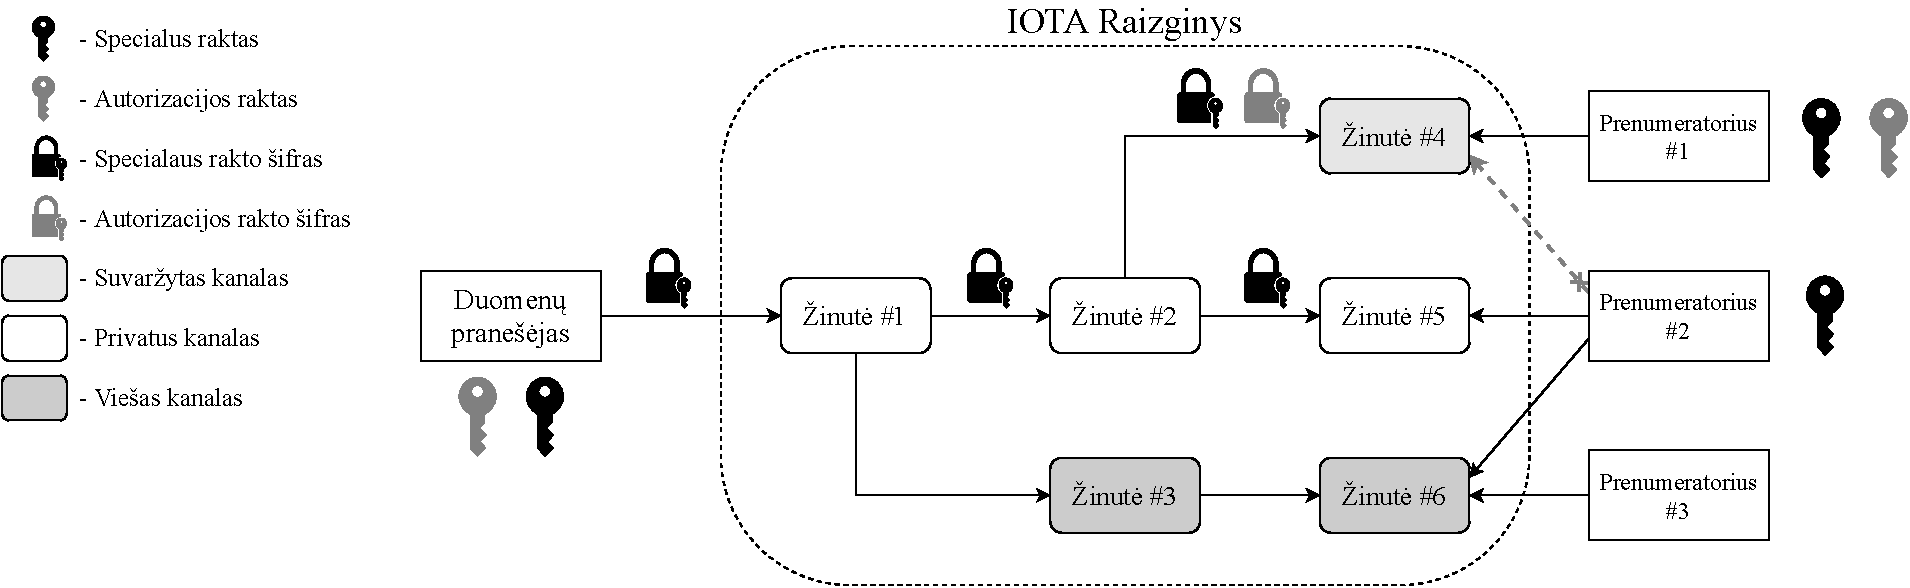
\includegraphics[scale=0.51]{images/mam-example}
    \caption{MAM supaprastintas modelis}
\end{figure}



% --------------------------------------------------------------- %
%               2.2.2.5. KVORUMU PAREMTI SKAIČIAVIMAI
% --------------------------------------------------------------- %

\subsubsubsection{Kvorumu paremti skaičiavimai}

Kaip jau nagrinėta 2.2.1.3 poskyryje, išmanieji kontraktai labai praturtina blokų grandines. Ne išimtis ir IOTA. To pagrindu IOTA platformoje kaip atskiras sluoksnis yra kuriamas kvorumu paremtų skaičiavimų protokolas, toliau – Qubic, sudarytas iš 3 esminių dedamųjų.

Pirmoji – orakulai (angl. \textit{Oracles}), atliekantys tinklo tarpininko su išoriniu pasauliu vaidmenį \cite{iota2017oracles}. Galimas to pavyzdys – IOTA tinklas negali žinoti nepamatuojamų įvykių, sukeltų gamtos stichijų, kitų tinklo narių ir t.t, kurių didelė dalis aprašyta straipsnyje \cite{behdani2012handle}. Orakulas šią informaciją galėtų surinkti ir transliuoti ją tinklui. Tačiau šia informacija orakulai gali manipuliuoti savo naudai. Kad to būtų išvengta, išorinio pasaulio faktų validumas turi būti priimtas kvalifikuota dauguma – kvorumu, t.y. ne mažiau nei 2/3 visų orakulų turi pateikti sutampančią informaciją \cite{iota2017oracles}. Taip pat egzistuoja ir kiti apsaugos mechanizmai, tokie kaip paskatos už teisingų rezultatų transliavimą, sankcijos už bandymus manipuliuoti informacija ir pan.

Antroji Qubic dedamoji – paskirstyti skaičiavimai \cite{iota2017oracles}. Daiktų internete smulkiems įrenginiams gali tekti susidurti su sudėtingais skaičiavimais, kurių šie įrenginiai nepajėgtų išspręsti arba tai užtruktų per daug laiko. Qubic protokolas įgalintų perduoti (angl. \textit{Outsource}) šiuos skaičiavimus išorinėms ir gerokai galingesnėms mašinoms, kurios grąžintų skaičiavimų rezultatus smulkiems įrenginiams.

Paskutinė Qubic protokolo dalis – išmanieji kontraktai. Išmanieji kontraktai pasižymi savybe: žinodami, kokius įvesties duomenis paduosime kontraktui, taip pat žinosime, kokio rezultato iš jo tikėtis \cite{iota2017oracles}. Ši savybė leidžia juos pritaikyti realizuojant mašinų tarpusavio bendravimą (angl. Machine to machine), toliau – M2M. Taip pat būtų galima automatizuoti informacijos apsikeitimą, bendravimą su prieš tai minėtais orakulais, bei paskirstytų skaičiavimų inicijavimą. Tačiau Qubic išmanieji kontraktai turi trūkumą: priešingai negu Ethereum platformoje, negalima atlikti automatizuotų finansinių pavedimų, nes tai yra neįmanoma architektūriškai.

Qubic įgyvendinimas iš dalies primena turimų akcijų konsensuso algoritmą (angl. \textit{Proof of Stake}), toliau – PoS, kurį turi įgyvendinę dalis blokų grandinių bei prie kurio ateityje ketina pereiti Ethereum platforma\footnote{Informacija iš: https://docs.ethhub.io/ethereum-roadmap/ethereum-2.0/proof-of-stake. Tikrinta 2019-05-14.}. PoS efektyvina tinklo naudojamus resursus, likviduodama PoW atliekamą darbą mašinoms bei pašalindama globalaus konsensuso poreikį smulkiems dalykams. Vietoje to, kad skaičiavimus bei balsavimą dėl visų išorinio pasaulio faktų atliktų kiekvienas tinkle esantis narys, šį darbą padaro specialūs agentai, IOTA platformoje vadinami orakulais.



% --------------------------------------------------------------- %
%               2.2.2.6. EKONOMINIS KLASTERIZAVIMAS
% --------------------------------------------------------------- %

\subsubsubsection{Ekonominis klasterizavimas}

Ekonominis klasterizavimas (angl. \textit{Economic Clustering}), toliau EC – samprata, pristatyta Sergey Ivancheglo ir įgalinanti IOTA platformos plečiamumą, kitaip - neribotą TPS kiekį \cite{sergey2018economic}.
Ekonominis klasteris – tai grupė prietaisų, esančių konkrečiame regione: kontinente, valstybėje, kelio ruože ar pastate \cite{sergey2018economic}. 

Pati idėja yra glaudžiai susijusi su daiktų internetu, o klasterių struktūra priklauso nuo ekonominės veiklos tame regione \cite{sergey2018economic}. IOTA platforma naudojasi vartotojai iš bet kurios pasaulio vietos, bet tai nėra efektyvu. Pavyzdžiui, JAV įsikūrusio fabriko temperatūros jutikliui nėra aktualu Kinijos piliečio transakcija savo draugui, gyvenančiam už kelių kvartalų. Tačiau jutiklis, norėdamas atlikdamas informacinę transakciją klientui, tikėtina, kad turės tvirtinti būtent jam neaktualią transakciją iš Kinijos. O juk būtų logiškiau, jeigu fabriko prietaisai turėtų prieigą tik prie jiems aktualių transakcijų.

EC išsidėstymo modelis pavaizduotas 10 pav. Kiekviename klasteryje yra lokaliai vykdomos IOTA transakcijos. Pavyzdžiui, 0 klasteris gali atlikti transakcijas 0 klasteryje, 1 klasteriui ir 2 klasteriui. Tačiau 0 ir 3 klasteris nėra kaimynai ir vienas kito transakcijų nemato, todėl jas ignoruoja. Jeigu iškiltų poreikis 0 klasterio nariui atlikti transakciją 3 klasteryje, šiam nariui tektų atlikti transakciją sau pačiam į 1 arba 2 klasterį, tada iš jo atlikti transakciją sau į 3 klasterį ir atlikti transakciją 3 klasteryje.

\begin{figure}[H]
    \centering
    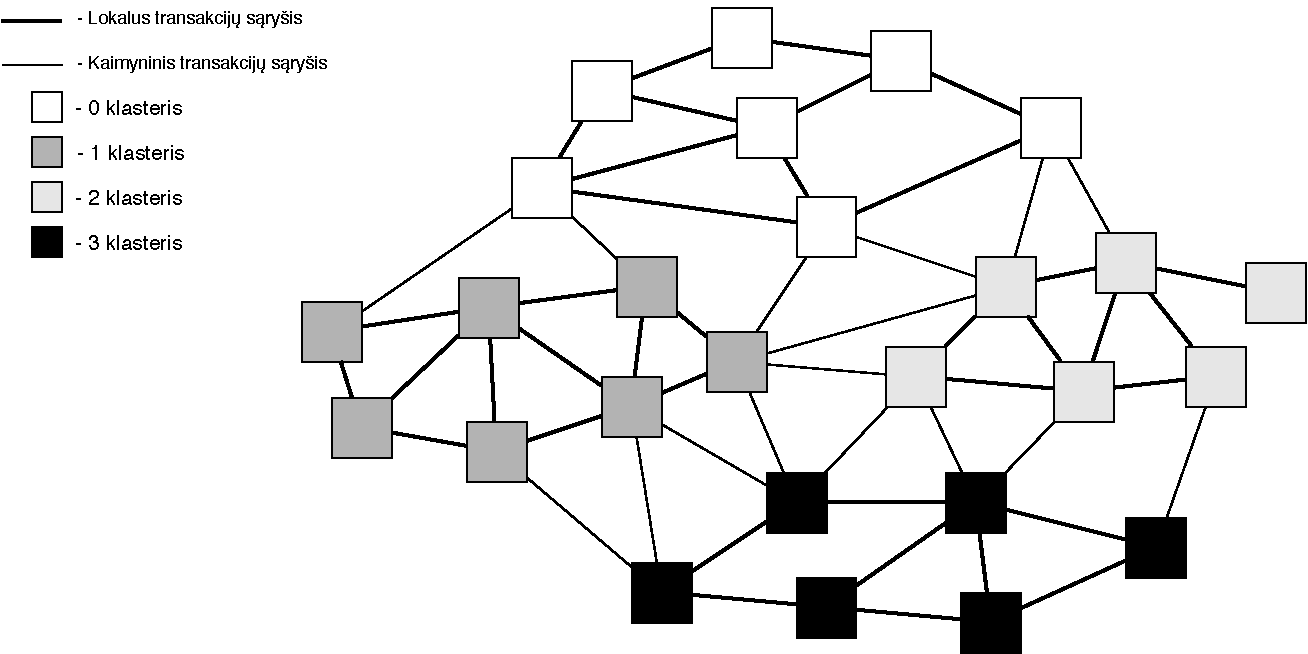
\includegraphics[scale=0.7]{images/economic-clusters}
    \caption{Ekonominio klasterizavimo modelis}
\end{figure}

Tačiau iš EC modelio kyla tam tikri trūkumai ir rizikos \cite{sergey2018economic}: 
\begin{itemize}
    \item Sunkumai atliekant transakcijas į tolimus klasterius;
    \item Dažnai tenka pervedinėti valiutą sau pačiam;
    \item Klasteriai gali kurti savo valiutą, kurios vertė kituose klasteriuose gali skirtis.
\end{itemize} 



% --------------------------------------------------------------- %
%            2.2.2.7. DALYVAVIMAS TINKLE NEPRISIJUNGUS
% --------------------------------------------------------------- %

\subsubsubsection{Dalyvavimas tinkle neprisijungus}

Transportuojant krovinius gali tekti atsidurti vietose, kuriose interneto ryšys yra nepasiekimas, taip pat reikia užtikrinti, kad darbas tęstųsi net ir trumpam dingus internetui. Pavyzdys – krovinių plukdymas per vandenyną. Naudojama technologija turi užtikrinti stabilų veikimą be interneto, ir kad atsiradus interneto ryšiui nebūtų pateikiami suklastoti duomenys.

Šiuo klausimu IOTA yra pranašesnė už Bitcoin ir Ethereum, nes įgalina transakcijas be interneto ryšio \cite{zivic2019distributed}. Transakcijų vykdymas periode be interneto pavaizduotas 11 pav. Vartotojas X, dingus internetui, mato visas transakcijas, išskyrus tas, kurias likęs tinklas atlieka nesant interneto ryšiui. Vienintelė logiška veiksmų seka vartotojui X yra susikurti savo atskirą raizginį (angl. \textit{sub-tangle}), kuriame X transakcijos tvirtins X transakcijas.

\begin{figure}[H]
    \centering
    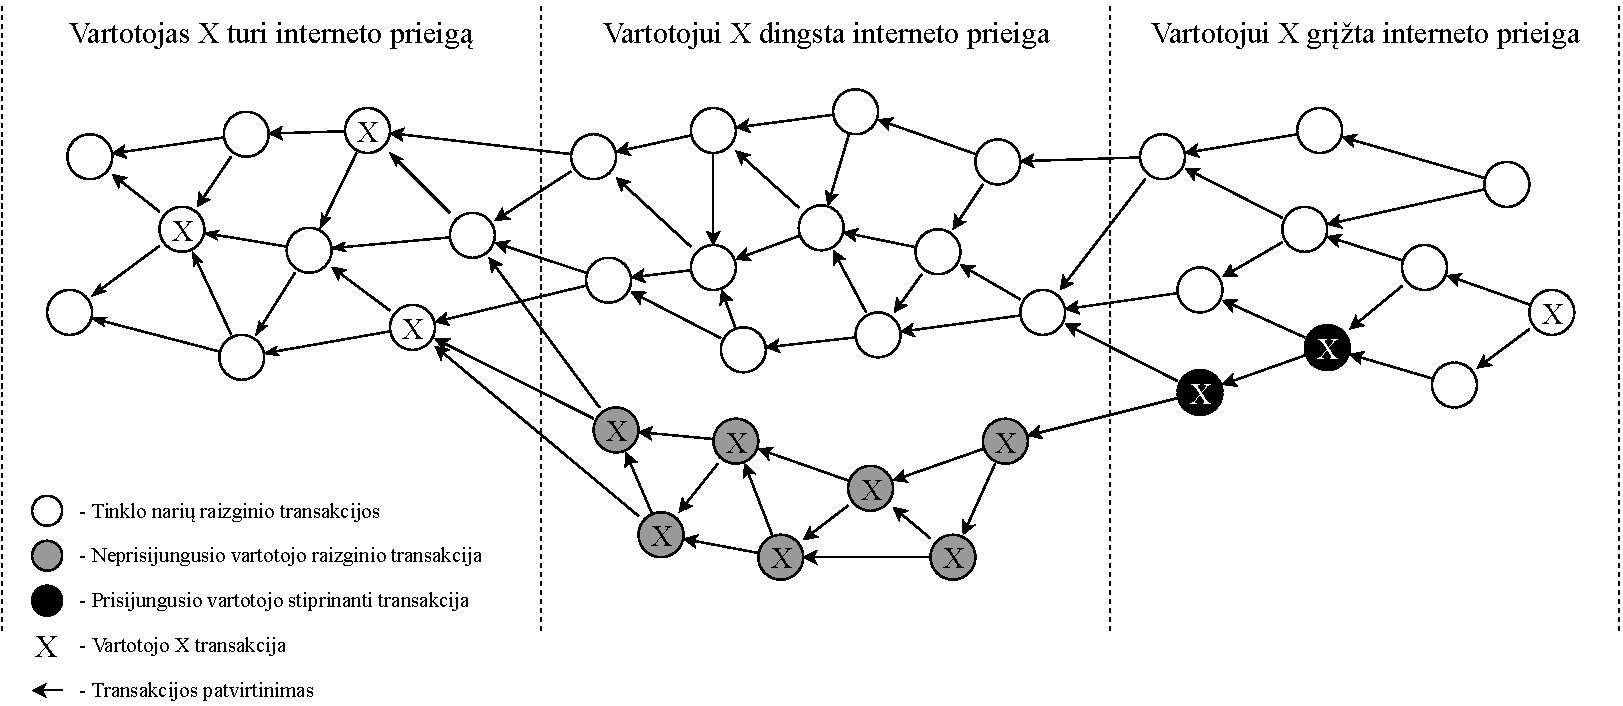
\includegraphics[scale=0.6]{images/offline-tangle}
    \caption{transakcijų vykdymas neturint interneto prieigos}
\end{figure}

Atsiradus interneto prieigai nereiškia, kad vartotojo X atskiras raizginys bus patvirtintas, todėl reikia atlikti specialias stiprinančias transakcijas, kurios padidina šansus, kad tinklas palaipsniui pripažins ir validuos atskirą raizginį kaip tinkamą įtraukti į bendrą tinklą \cite{bennet2017technical}. Stiprinanti transakcija būtinai turi patvirtinti vieną pagrindinio raizginio ir vieną atskiro raizginio X transakciją \cite{bennet2017technical}. Kuo daugiau stiprinančių transakcijų, tuo didesnė validavimo tikimybė, tačiau yra reikalingos bent 2 stiprinančios transakcijos \cite{bennet2017technical}.



% --------------------------------------------------------------- %
%              2.3. BLOKŲ GRANDINĖS IR DAG PALYGINIMAS
% --------------------------------------------------------------- %

\subsection{Blokų grandinės ir DAG palyginimas}

Taigi, galima apibendrinti pagrindinius skirtumus tarp DAG ir blokų grandinių principais paremtas DLT. Architektūra yra akivaizdžiausias skirtumas. Blokų grandinė yra tiesinės formos darinys, sudarytas iš nuosekliai sujungtų blokų, o DAG yra raizginys, sudarytas iš individualių transakcijų. Tačiau iš to kyla IOTA trūkumas – palankesnės sąlygos piktybinių transakcijų (angl. \textit{Spam}) kūrimui. Blokų grandinėse sukurti atskirą piktybinių blokų atšaką yra gerokai sudėtingiau ir reikalauja daugiau resursų negu kuriant atskirą transakcijų grandį IOTA tinkle. Tačiau nuogąstauti dėl tinklo pažeidžiamumo nėra pagrindo. Tam, kad būtų pažeistas duomenų stabilumas, abiem atvejais kenkėjo skaičiavimo resursai turi būti didesni nei viso likusio tinklo.

Abi DLT atmainos naudoja PoW skaičiavimus, tačiau IOTA tinkle kiekvienas narys juos atlieka individualiai. Tuo tarpu blokų grandinėse šį procesą galime deleguoti. Esant aukštam PoW skaičiavimų sudėtingumui, tai tampa trūkumu tiekimo grandinėse. Jeigu daiktų internetas taptų visuotinai naudojama technologija logistikoje, transakcijas arba apsikeitimą duomenimis turėtų atlikti net ir patys smulkiausi prietaisai, nepasižymintys didele skaičiavimo galia.

Dar vienas IOTA trūkumas yra koordinatorius. Šiuo metu pastaroji pltforma yra ankstyvoje fazėje ir negali savarankiškai funkcionuoti, todėl ją turi prižiūrėti specialus agentas, vadinamas koordinatoriumi \cite{bramas2018stability}. Yra teigiama, kad tai pažeidžia vieną iš pagrindinių DLT principų – nepriklausomumą nuo trečiųjų šalių. Šiuo atžvilgiu blokų grandinės lenkia IOTA, nes gali veikti autonomiškai, be trečiosios šalies įsikišimo. Vis dėlto IOTA kūrėjai ateityje tikisi pašalinti koordinatoriaus poreikį \cite{bramas2018stability}.

Saugumo klausimu IOTA turi pranašumą kvantinių kompiuterių atžvilgiu, tačiau tai yra labiau aktualu ilgojoje perspektyvoje. Kol kas nėra sukurtų galingų, pigių ir plačiai naudojamų kvantinių kompiuterių, todėl šis privalumas šiandien nėra lemiamas veiksnys renkantis tarp šių dviejų DLT tipų. Be to, blokų grandinės laikui bėgant galėtų prisitaikyti prie kvantinių kompiuterių keliamų grėsmių pakeisdamos savo architektūrinius sprendimus.

Ko gero didžiausią įtaką technologijos pasirinkimui lemia rodikliai, susiję su atliekamų transakcijų greičiu ir kaina. Tiekimo grandinėms yra svarbu, kad transakcijos apsimokėtų, t.y. įvyktų kuo greičiau ir pigiau. Svarbu lyginti rodiklius, darančius įtaką maksimaliai tinklo apkrovai, vienos transakcijos įvykdymo laikui ir piniginiam naudingumui. Didžioji dalis blokų grandinių turi TPS limitus arba transakcijos mokestį, o IOTA – ne. Taigi, pritaikius IOTA tiekimo grandinėse, būtų galima dalintis informacija už dyką ir labai greitai, sutaupant daug resursų visuose grandies procesuose.

IOTA taip pat įgalina transakcijas neprisijungus ir MAM, sukuriančius potencialių technologijos panaudojimo atvejų, o pilnai įgyvendinus kvorumu paremtus skaičiavimus ir ekonominį klasterizavimą, jų atsirastų dar daugiau.

Nepaisant visų IOTA trūkumų, remdamasis jos pranašumais blokų grandinių atžvilgiu ir sąlygomis daiktų internetui autorius daro prielaidą, jog būtent ši DLT atmaina yra palankesnė taikymui tiekimo grandinių ir logistikos srityje. 